\section{Descripción del Problema}\label{descripciuxf3n-del-problema}

Se consideraá una empresa dedicada a la venta y renta de inmuebles cuyos canales  de venta són  entrevistas y mediante llamadas telefónicas. Ha decidido invertir en un sitio web donde publica el listado de propiedades a ofertar. Como en la mayoria de sitios web el diseño se centra unicamente en ser un portal informativo y poca interacción con el usuario. Por consecuencia los clientes que visitan el sitio (ver info de visitas) observan que resulta muy complicado localizar alguna propiedad relevante. O las que se muestran como relevantes están fuera de su presupuesto.

Este ejemplo es el caso de la mayoria de negocios mexicanos que utilizan un portal web para anunciarse y no aprovechan la interacción con sus clientes.
Dentro de la ciudad de Morelia, se han detectado poco más de 30 inmobiliarias que utilizan portales para promoción, incluso las principales constructoras (Arko, Habicasa) utilizan  portales de tipo informativo. Este proyecto busca incrementar la cantidad de información que un usuario promedio recibe al consultar una propiedad incluyendo opciones similares con el fin de mantener el usuario más tiempo en sitio y por consecuencia incrementar la utilidad de la información. Durante la navegación se buscará conocer al usuario a través de breves cuestionarios sobre la información que se está consultando para identificar potenciales opciones. 

\subsection{Metodología}

Nuestra propuesta de diseño se centra en 4 puntos.
\begin{enumerate}
\item Crear un Marco de Datos, recopilando información de inmobiliarias de la ciudad de Morelia.
\item Identificar usuarios potenciales que deseen adquirir propiedades.
\item Proporcionar sugerencias cercanas a las deseadas.
\item Medir la precisión a través de encuestas de satisfacción al cliente.
\end{enumerate}


\subsection{Recolección de los datos}

Para la recolección se  utilizo un crawler publico{[}6{]} que indexa las paginas web de las inmobiliarias, de ahí obtenemos una lista de links (ver figura 1), filtramos la lista dejando unicamente las que se refieren a propiedades y almacenanos los documentos en HTML. Extraemos el corpus con python y almacenamos cada propiedad en el dataset para convertirlo a un archivo csv con el cual realizaremos la clasificación de las propiedades.
\begin{figure}[h]
\centering
\begin{tabular}{cc}
  \hline
 & Total \\ 
  \hline
Bodega &   5 \\ 
  Casa & 168 \\ 
  Departamento &  24 \\ 
  Edificio &   1 \\ 
  Local &  13 \\ 
  Oficinas &   1 \\ 
  Terreno &  72 \\ 
   \hline
\end{tabular}
\caption{Tabla de Propiedades por Inmueble}
\end{figure}


\begin{figure}[htbp]
\centering
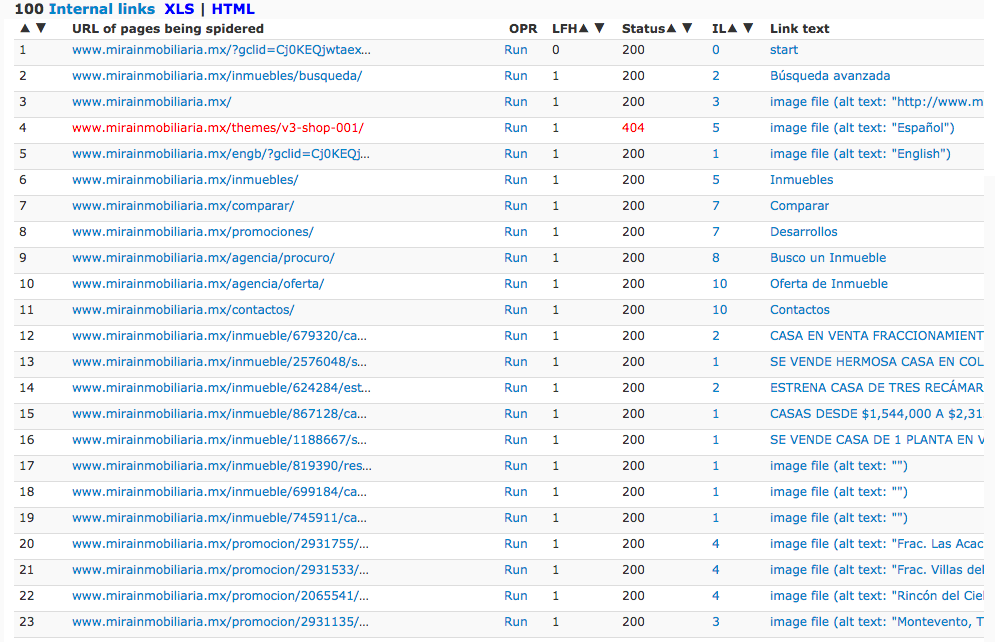
\includegraphics[width=0.8\textwidth]{CrawlerSite.png}
\caption{Listado de Artículos relacionados con propiedades}
\end{figure}

\begin{figure}[htbp]
\centering
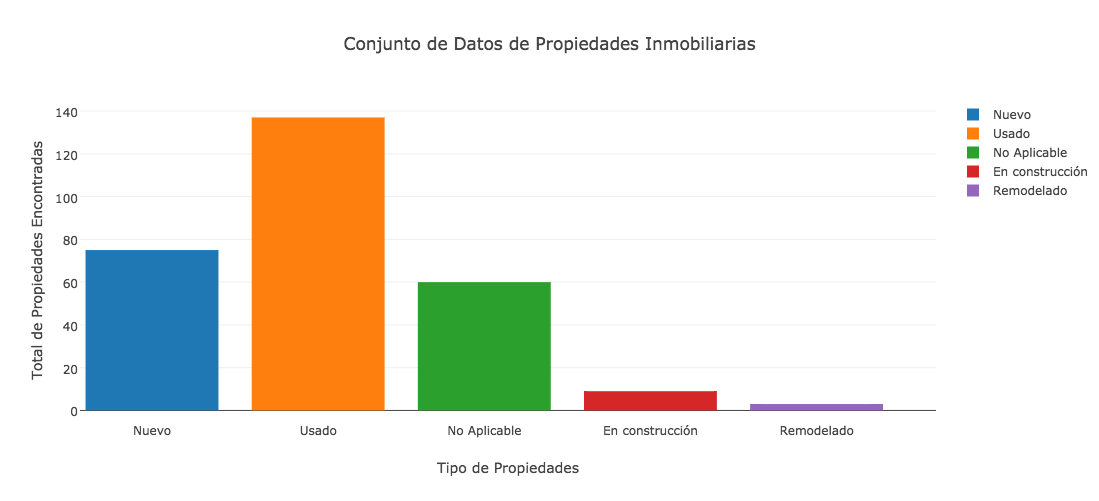
\includegraphics[width=0.8\textwidth]{PropiedadesInmobiliariasEstadoVivienda.png}
\caption{Distribución de Propiedades Tipo de Propiedad}
\end{figure}

\subsection{Clasificación de las propiedades}
Para el procesamiento de los datos decidimos utilizar el lenguaje de programación R, para analizar y clasificar. Las propiedades que descargamos de los web sites las hemos agrupado en un solo listado con aproximadamente 500 propiedades, las cuales  vienen listadas por Estado (Usado, Nuevo, Construcción), Área construida ($m^2$), Zona (Colonia o barrio de Referencia), Precio, Latitud, Longitud y algunas otras características deseadas.  El algoritmo de clasificación para esta sección que hemos seleccionado es el de vecinos cercanos ya que estamos trabajando con variables categóricas, nuestro objetivo es analizar si podemos definir clases de propiedades.
\begin{figure}[htbp]
\centering
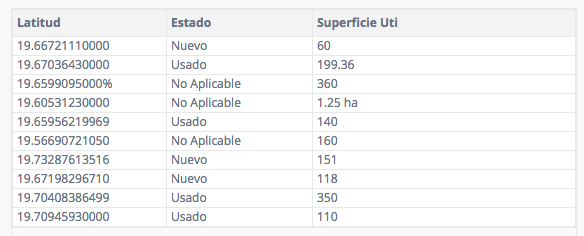
\includegraphics[width=0.8\textwidth]{Dataset.png}
\caption{Dataset de Propiedades Inmobiliarias}
\end{figure}


\subsection{KNN - Nearest Neighbor}
También conocido como K-nearest Neighbor es el más simple de los algoritmos de aprendizaje máquina que existe y el más utilizado. Se basa en identificar los k  registros en el conjunto de entrenamiento que son "cercanos" en similaridad. La prueba asigna una clase a la mayoria de los vecinos cercanos. El K-NN trata las caracteristicas como coordenadas multidimensionales. Para ejemplo tomamos las características de un conjunto de prueba que definimos como ingredientes. El algoritmo requiere un conjunto entrenamiento y un conjunto prueba, en nuestro caso usamos para entrenamiento únicamente las casas con estado = 'usado'.

\subsection{Metrica de similaridad con distancia.}

El Knn requiere una función distancia, o una fórmula que mida la similaridad entre dos instancias. Existen diferentes maneras de calcular la distancia. Tridicionalmente el Knn utiliza la distancia euclideana, que es la distancia de un punto con respecto a otro conectados por una linea o regla. La distancia euclideana se expresa de la siguiente manera:
\begin{equation}
dist(x,y) = \sqrt{(p_1-q_1)^2 + (p_2-q_2)^2+ \cdots + (p_n - q_n)^2}
\end{equation}

La desición de cuantos vecinos cernanos para el uso de K-NN determina que tan bien el modelo generaliza para futuros datos. El balance entre sobre ajustar o subajustar el conjunto de entrenamiento es un problema conocido como Ajuste de la varianza. Seleccionando valores de K reduce el impacto de la varianza causada por datos ruidosos, pero puede que el sistema ignore los grupos pequeños, pero importante patrones. En el lado opuesto usando una k mayor se influye sobre la muestra clasificada. Obviamente, el mejor valor de k se encuentra entre estos dos extremos.
\begin{figure}[h]
\centering
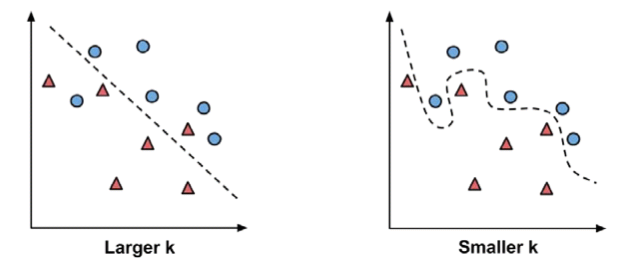
\includegraphics[width=0.5\textwidth]{IMG_0061.png}
\caption{Selección de la k en KNN}
\end{figure}


